\subsection{Shell-Sort Algorithm:}

For the following algorithm we create a {\itshape Class} with the name of the algorithm, in its constructor will receive as parameters only the list to sort, this list has the name of {\itshape dimensions} as we can see in line 3, in line 4 the program corroborates that the length of {\itshape dimensions} it's bigger than 1, in case that do not accomplish the condition then the program stops running because there is no need of sorting, otherwise the program continues running and in line 6 and 7 stores in a instance of the class the length of {\itshape dimensions} and the {\itshape gap} value, that is the length divided by 2, this three variables are going to be used along the execution. \hfill \break

The shell sort, sometimes called the "diminishing increment sort", improves on the insertion sort by breaking the original list into a number of smaller sub-lists, each of which is sorted using an insertion sort. The unique way that these sub-lists are chosen is the key to the shell sort. Instead of breaking the list into sub-lists of contiguous items, the shell sort uses an increment {\itshape i} sometimes called the {\bfseries gap}  to create a sub-list by choosing all items that are {\itshape i} item apart.  \hfill \break

This can be seen in Figure 3.3.0. This list has nine items. If we use an increment of three, there are three sublists, each of which can be sorted by an insertion sort. After completing these sorts, we get the list shown in Figure 3.3.1. Although this list is not completely sorted, something very interesting has happened. By sorting the sublists, we have moved the items closer to where they actually belong. \hfill \break

\begin{figure}[H]
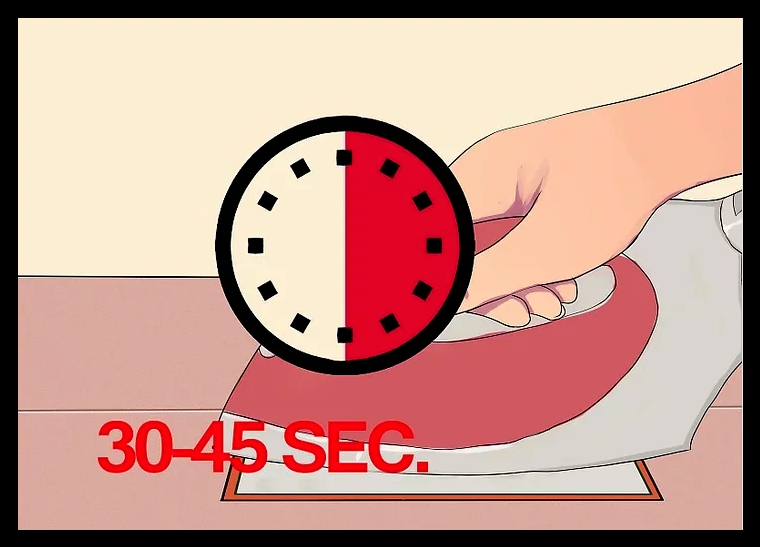
\includegraphics[width = 16.5cm, height = 5cm]{2.png}
\centering \linebreak \linebreak {\small Figure 3.3.0: Initial sub-lists.}
\end{figure}

\begin{figure}[H]
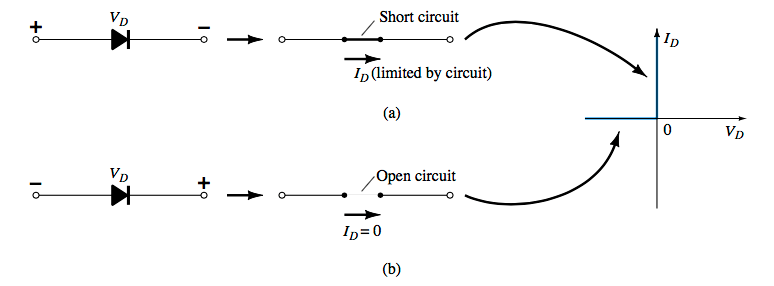
\includegraphics[width = 16.5cm, height = 4cm]{3.png}
\centering \linebreak \linebreak {\small Figure 3.3.1: Sorting sub-lists.}
\end{figure} 

Figure 3.3.2 shows a final insertion sort using an increment of one; in other words, a standard insertion sort. Note that by performing the earlier sublist sorts, we have now reduced the total number of shifting operations necessary to put the list in its final order. For this case, we need only four more shifts to complete the process. \hfill \break

\begin{figure}[H]
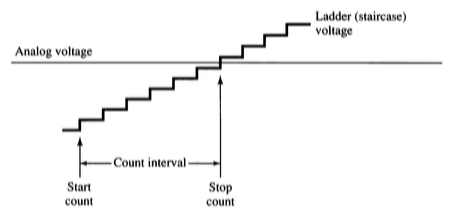
\includegraphics[width = 16.5cm, height = 4cm]{4.png}
\centering \linebreak \linebreak {\small Figure 3.3.2: Swapping elements.}
\end{figure} 

The previous procedure can be implemented in the code below: \hfill \break

\begin{lstlisting}
class Shell:
    # Class constructor.
    def __init__ ( self, dimensions ):
        assert len ( dimensions ) > 1
        self.dimensions = dimensions
        self.n = len ( dimensions )
        self.gap = int ( self.n / 2 )

    # Shellsort algorithm.
    def shellsort ( self ):
        # Do a gapped insertion sort for the gap size.
        # The first gap elements of dimensions [ 0 .. gap - 1 ] are already in
        # gapped order then, keep adding one more element until the entire array
        # is gap sorted.
        while ( self.gap > 0 ):
            # Add dimensions [ i ] to the elements that have been gap sorted.
            for i in range ( self.gap, self.n ):
                # Save dimensions [ i ] in the variable 'temp', and make a hole
                # at i position.
                temp = self.dimensions [ i ]
                # Shift earlier gap-sorted elements up until the correct location
                # for dimensions [ i ] is found.
                j = i
                while ( j >= self.gap and self.dimensions [ j - self.gap ] > temp ):
                    self.dimensions [ j ] = self.dimensions [ j - self.gap ]
                    j = j - self.gap
                # Put 'temp' ( the original dimensions [ i ] ) in its correct location.
                self.dimensions [ j ] = temp
            self.gap = int ( self.gap / 2 )
\end{lstlisting}

\pagebreak